% =====================================================================
%  Lab 1 report -- Cristian, NTP, Lamport + vector clocks, Ricart-Agrawala
%
%  Build:   cd report/stanleyreport && latexmk -pdf main.tex
%  Clean:   latexmk -C
%
%  How this template is organised
%    preamble.tex                  packages + helper macros (\TODO, \src, ...)
%    sections/00-overview.tex      environment, protocol list, conventions
%    sections/01-cristian.tex      §3.1 of LAB1.en.md
%    sections/02-ntp.tex           §3.2
%    sections/03-logical-clocks.tex  §3.4
%    sections/04-ricart-agrawala.tex §4.4
%    sections/05-summary.tex       cross-protocol comparison, lessons, bonus
%    sections/A-reproduce.tex      appendix: index of runs / JSON / figures
%    figures/                      put your space-time-diagram screenshots here
%
%  Every protocol section has the same shape (what LAB1 §2.1 and §6.2 ask):
%    algorithm -> implementation -> scenario coverage table ->
%    normal / fault A (crash) / fault B (partition or latency) /
%    extra handout scenarios / design variant -> discussion -> boundaries
% =====================================================================
\documentclass[11pt,a4paper]{article}
% =====================================================================
%  preamble.tex -- packages, colours and helper macros for the report.
%  You normally do not need to edit this file; edit main.tex instead.
% =====================================================================

\usepackage[margin=2.2cm]{geometry}
% lmodern = scalable fonts.  If it is not installed (e.g. a minimal TeX Live),
% fall back to the default fonts and skip microtype, which needs scalable fonts.
\IfFileExists{lmodern.sty}
  {\usepackage[T1]{fontenc}\usepackage{lmodern}\usepackage{microtype}}{}
\usepackage[utf8]{inputenc}
\usepackage{amsmath,amssymb}
\usepackage{booktabs,tabularx,array,multirow}
\usepackage{graphicx}
\usepackage{float}
\usepackage{caption,subcaption}
\usepackage[dvipsnames]{xcolor}
\usepackage{enumitem}
\usepackage{listings}
\usepackage{tikz}
\usetikzlibrary{arrows.meta,positioning,calc}
\usepackage[most]{tcolorbox}
\usepackage{fancyhdr}
\usepackage{siunitx}
\usepackage[colorlinks=true,linkcolor=accent,urlcolor=RoyalBlue,citecolor=accent]{hyperref}
\usepackage{xurl} % lets long paths/URLs break at any character

% ---------------------------------------------------------------------
%  Colours
% ---------------------------------------------------------------------
\definecolor{accent}{HTML}{1F4E79}
\definecolor{codebg}{HTML}{F5F5F5}

% ---------------------------------------------------------------------
%  Page style
% ---------------------------------------------------------------------
\pagestyle{fancy}
\fancyhf{}
\fancyhead[L]{\small Lab 1 -- Visualizing Distributed Protocols}
\fancyhead[R]{\small\nouppercase{\leftmark}}
\fancyfoot[C]{\thepage}
\setlength{\headheight}{14pt}
\setlength{\parskip}{0.4em}
\setlength{\parindent}{0pt}

% ---------------------------------------------------------------------
%  TODO markers.  Set \showtodosfalse in main.tex before submitting:
%  every \TODO{...} and \fillin then disappears from the PDF.
% ---------------------------------------------------------------------
\newif\ifshowtodos
\showtodostrue
\newcommand{\TODO}[1]{\ifshowtodos\leavevmode{\color{red}\textbf{[TODO:} #1\textbf{]}}\fi}
\newcommand{\fillin}{\ifshowtodos\leavevmode{\color{red}\rule{1.6em}{0.4pt}}\fi}

% ---------------------------------------------------------------------
%  Links into the repository.
%  \src{protocols/christian/protocol.go} prints the path and links to it
%  on GitHub.  Change \repobranch if your code lives on another branch.
% ---------------------------------------------------------------------
\newcommand{\repobase}{https://github.com/stanleyyoeng44-sketch/distvis}
\newcommand{\repobranch}{main}
\newcommand{\src}[1]{\href{\repobase/blob/\repobranch/#1}{\nolinkurl{#1}}}
% exported run records (Run history -> Export record) live in report/
\newcommand{\jsonfile}[1]{\src{report/#1}}

% field / method names, e.g. \fld{lastSync.errorAfterMs}
\newcommand{\fld}[1]{\texttt{\detokenize{#1}}}

% ---------------------------------------------------------------------
%  Scenario layout helpers
% ---------------------------------------------------------------------
% \scenario{Title}{label}  -> a numbered subsection with a label sec:label
\newcommand{\scenario}[2]{\subsection{#1}\label{sec:#2}}
% bold run-in heading inside a scenario ("Setup", "Steps", ...)
\newcommand{\phead}[1]{\par\medskip\noindent{\color{accent}\textbf{#1}}\par\nopagebreak}

% two-column table describing the experiment settings
\newenvironment{setuptable}
  {\par\smallskip\noindent\small\tabularx{\linewidth}{@{}>{\bfseries}p{3.6cm}X@{}}\toprule}
  {\bottomrule\endtabularx\par\smallskip}

% numbered reproduction steps
\newlist{steps}{enumerate}{1}
\setlist[steps]{label=\arabic*.,leftmargin=*,itemsep=1pt,topsep=2pt}

% \screenshot[width]{file.png}{caption}
% If figures/file.png does not exist yet, a grey placeholder box is drawn,
% so the report always compiles.
\newcommand{\screenshot}[3][0.95\linewidth]{%
  \begin{figure}[H]\centering
    \IfFileExists{figures/#2}%
      {\includegraphics[width=#1]{figures/#2}}%
      {\fcolorbox{gray}{gray!5}{\parbox[c][4.2cm][c]{#1}{\centering\color{gray}%
        Screenshot placeholder\\[2pt]\small put \nolinkurl{figures/#2} here}}}%
    \caption{#3}\label{fig:#2}
  \end{figure}}

% discussion question box: \begin{qa}{question text} answer \end{qa}
\newtcolorbox{qa}[1]{breakable,enhanced,colback=gray!3,colframe=accent!70,
  fonttitle=\bfseries,title={#1},left=6pt,right=6pt,top=4pt,bottom=4pt}

% grey "how to use this section" note (hidden together with TODOs)
\newcommand{\hint}[1]{\ifshowtodos\par{\small\color{gray}\textit{Hint: #1}}\par\fi}

% ---------------------------------------------------------------------
%  Code listings (Go)
% ---------------------------------------------------------------------
\lstdefinelanguage{Go}{
  morekeywords={break,case,chan,const,continue,default,defer,else,fallthrough,
    for,func,go,goto,if,import,interface,map,package,range,return,select,struct,
    switch,type,var,nil,true,false,int64,string,error,bool},
  sensitive=true, morecomment=[l]{//}, morecomment=[s]{/*}{*/},
  morestring=[b]", morestring=[b]`}
\lstset{basicstyle=\ttfamily\small,backgroundcolor=\color{codebg},
  keywordstyle=\color{accent}\bfseries,commentstyle=\color{gray}\itshape,
  stringstyle=\color{OliveGreen},frame=single,rulecolor=\color{gray!40},
  breaklines=true,columns=fullflexible,showstringspaces=false,
  numbers=left,numberstyle=\tiny\color{gray}}

% ---------------------------------------------------------------------
%  Space-time diagram helpers (TikZ)
%  \proc{y}{name}{xmax}  draws one process line at height y
% ---------------------------------------------------------------------
\tikzset{
  msg/.style={-{Stealth[length=2.2mm]},thick,accent},
  ev/.style={circle,fill=black,inner sep=1.4pt},
  lbl/.style={font=\scriptsize},
}
\newcommand{\proc}[3]{%
  \draw[gray,thick] (0,#1) node[left,black]{\small #2} -- (#3,#1);}


% ------------------------- fill these in -----------------------------
\newcommand{\authorname}{Stanley \TODO{full name}}
\newcommand{\studentid}{\TODO{student ID}}
\newcommand{\coursename}{Operating Systems and Distributed Systems}
\newcommand{\submitdate}{\today}

% Set to \showtodosfalse to hide every red TODO / blank / hint before submitting.
\showtodostrue
% ---------------------------------------------------------------------

\begin{document}

\begin{titlepage}
  \centering
  \vspace*{3cm}
  {\Large \coursename\par}
  \vspace{1cm}
  {\Huge\bfseries Lab 1: Visualizing Distributed Protocols\par}
  \vspace{0.6cm}
  {\Large Cristian $\cdot$ NTP $\cdot$ Lamport \& vector clocks $\cdot$ Ricart--Agrawala\par}
  \vspace{2cm}
  {\large \authorname\par}
  {\large \studentid\par}
  \vfill
  {\large \submitdate\par}
\end{titlepage}

\tableofcontents
\clearpage

\section{Overview}

\subsection{Goal of this report}
This report covers my part of Lab~1 (\src{docs/LAB1.en.md}): four protocols, each
implemented as a Go module in \nolinkurl{protocols/} and run on the DistVis platform.
For every protocol I show the normal behaviour, a crash scenario, a partition or
high-latency scenario, and a design variant, as required by §2.1 of the handout.

\TODO{One or two sentences: which teammates cover the remaining required protocols
(Berkeley, Bully, Lamport mutual exclusion, 2PC, \dots) and where their part is.}

\begin{table}[H]\centering\small
\begin{tabularx}{\linewidth}{@{}llXl@{}}
\toprule
Module & Protocol & Code directory & Handout \\
\midrule
L03 Clocks & Cristian          & \src{protocols/christian}      & §3.1 \\
L03 Clocks & NTP               & \src{protocols/ntp}            & §3.2 \\
L03 Clocks & Lamport + vector  & \src{protocols/logical-clocks} \TODO{or \nolinkurl{protocols/lamport}?} & §3.4 \\
L04 Mutual exclusion & Ricart--Agrawala & \src{protocols/randa} & §4.4 \\
\bottomrule
\end{tabularx}
\caption{Protocols covered in this report.}
\end{table}

\subsection{Environment}
\begin{setuptable}
Platform     & DistVis, started with \texttt{npm start}, UI at \url{http://localhost:3000} \\
Node.js      & \TODO{version} \\
Go           & \TODO{version} \\
Docker       & \TODO{version} \\
Runtime mode & Docker (real Go nodes) for every result in this report, unless stated otherwise \\
Machine / OS & \TODO{CPU, OS} \\
\end{setuptable}

\hint{The built-in simulation does not run your Go code (LAB1 §1.3). Say clearly
which mode each run used.}

\subsection{How the evidence is presented}
\begin{itemize}[itemsep=2pt]
  \item \textbf{Space-time diagrams.} Screenshots from the platform. Horizontal axis
        is time, one row per node; solid arrow = delivered message, dashed = in flight,
        red $\times$ = dropped, coloured square = a \fld{node.Report(...)} state report.
  \item \textbf{Exported runs.} JSON files from ``Run history $\rightarrow$ Export record'',
        stored in \src{report}. Each scenario names its file.
  \item \textbf{Automated scenarios.} Where a protocol has a \nolinkurl{scenarios.json},
        the scenario can be replayed with
        \texttt{node scripts/scenarios.mjs run <protocol> <scenario-id>}
        (\src{scripts/scenarios.mjs}).
\end{itemize}

\subsection{Conventions}
\begin{itemize}[itemsep=2pt]
  \item \fld{errorMs} = (node's simulated clock) $-$ (real time), in milliseconds.
        Positive means the node is ahead. The algorithms never read it; it exists only
        so an observer can judge accuracy.
  \item Nodes are called \texttt{node-1}, \dots, \texttt{node-n}. Link delays are written
        \texttt{node-a$\to$node-b = 200\,ms} (one direction only unless stated).
  \item \TODO{any other convention you use, e.g.\ rounding of numbers}
\end{itemize}

\clearpage
\section{Cristian clock synchronization}\label{sec:cristian}
Handout: LAB1 §3.1 \\
Code: \src{protocols/christian} \\
README: \src{protocols/christian/README.md}

% ---------------------------------------------------------------------
\subsection{Algorithm}
A client reads its clock ($T_0$), asks the time server for the time, receives the
server's reading $T_s$, and reads its clock again ($T_1$). It then sets
\[
  C \leftarrow T_s + \frac{T_1 - T_0}{2}, \qquad
  \text{worst-case error} \le \frac{T_1 - T_0}{2} = \frac{\mathrm{RTT}}{2}.
\]

\begin{figure}[H]\centering
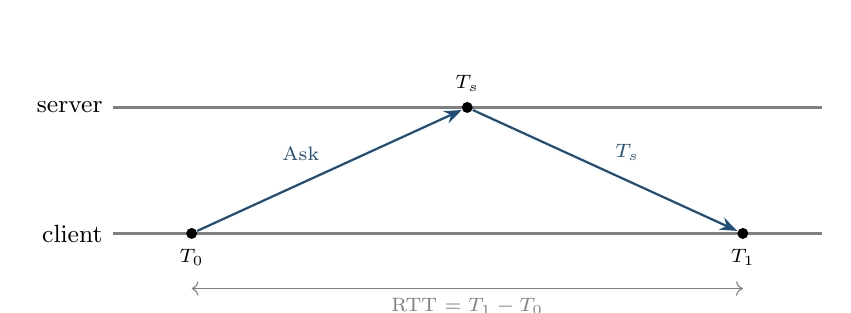
\begin{tikzpicture}[x=1cm,y=1cm]
  \proc{1.6}{server}{9}
  \proc{0}{client}{9}
  \node[ev,label=below:{\scriptsize $T_0$}] (t0) at (1,0) {};
  \node[ev,label=above:{\scriptsize $T_s$}] (ts) at (4.5,1.6) {};
  \node[ev,label=below:{\scriptsize $T_1$}] (t1) at (8,0) {};
  \draw[msg] (t0) -- node[lbl,above left]{Ask} (ts);
  \draw[msg] (ts) -- node[lbl,above right]{$T_s$} (t1);
  \draw[<->,gray] (1,-0.7) -- node[below,lbl]{RTT $=T_1-T_0$} (8,-0.7);
\end{tikzpicture}
\caption{One Cristian round.}
\end{figure}

\TODO{2--4 sentences in your own words: why the midpoint, and what assumption
(symmetric delay) the formula depends on.}

% ---------------------------------------------------------------------
\subsection{Implementation}
\begin{itemize}[itemsep=2pt]
  \item Formula: \TODO{function name} in \src{protocols/christian/protocol.go}
  \item Client side (one \fld{Sync}): \TODO{} \quad Server side (\fld{TimeService.Ask}): \TODO{}
  \item Simulated clock (offset + drift): \src{protocols/christian/clock.go}
  \item Automated scenarios: \src{protocols/christian/scenarios.json}
\end{itemize}

\phead{State fields reported}
\begin{table}[H]\centering\small
\begin{tabularx}{\linewidth}{@{}lX@{}}
\toprule
Field & Meaning \\ \midrule
\fld{role}              & \TODO{} \\
\fld{errorMs}           & \TODO{} \\
\fld{driftPPM}          & \TODO{} \\
\fld{syncs} / \fld{failedSyncs} & \TODO{} \\
\fld{lastSync}          & \TODO{($t_0$, $T_s$, $t_1$, RTT, estimate, correction, error bound, error before/after)} \\
\fld{lastError}         & \TODO{} \\
\bottomrule
\end{tabularx}
\end{table}

\phead{Application inputs}
\begin{table}[H]\centering\small
\begin{tabularx}{\linewidth}{@{}llX@{}}
\toprule
Input & Fields & Effect \\ \midrule
\fld{Application.Sync}           & \fld{server}, \fld{mode} & \TODO{} \\
\fld{Application.SetServerDelay} & \fld{delayMs}            & \TODO{} \\
\fld{Application.SetClock}       & \fld{offsetMs}, \fld{driftPPM} & \TODO{} \\
\bottomrule
\end{tabularx}
\end{table}

% ---------------------------------------------------------------------
\subsection{Scenario coverage}
\begin{table}[H]\centering\small
\begin{tabularx}{\linewidth}{@{}llXl@{}}
\toprule
Report section & Handout & What it shows & Export \\ \midrule
\ref{sec:cr-normal}  & A          & symmetric sync, error $\to 0$ & \nolinkurl{cristian_scenA_normal.json} \\
\ref{sec:cr-crash}   & (fault A)  & time server crashes           & \nolinkurl{cristian_scenB_crash.json} \\
\ref{sec:cr-asym}    & B          & asymmetric link               & \nolinkurl{cristian_scenC_asymmetric.json} \\
\ref{sec:cr-queue}   & C          & server queuing delay          & \nolinkurl{cristian_scenD_serverDelay.json} \\
\ref{sec:cr-variant} & variant    & $+0$ vs $+\mathrm{RTT}/2$ vs $+\mathrm{RTT}$ & \nolinkurl{cristian_designVariant.json} \\
\bottomrule
\end{tabularx}
\end{table}

% ---------------------------------------------------------------------
\scenario{Normal: one sync over symmetric links}{cr-normal}
\phead{Setup}
\begin{setuptable}
Nodes / latency & 3 nodes, \TODO{80}\,ms, Docker \\
Scenario id     & \texttt{a-normal} \\
Export          & \jsonfile{cristian_scenA_normal.json} \\
\end{setuptable}
\phead{Steps}
\begin{steps}
  \item Record the initial \fld{errorMs} of every node.
  \item On node-2 run \fld{Application.Sync} with \fld{server=node-1}, \fld{mode=half}.
  \item \TODO{}
\end{steps}
\phead{Result}
\begin{table}[H]\centering\small
\begin{tabular}{@{}lrrrrr@{}}
\toprule
Node & errorBefore (ms) & RTT (ms) & correction (ms) & errorAfter (ms) & bound (ms) \\ \midrule
node-2 & \fillin & \fillin & \fillin & \fillin & \fillin \\
node-3 & \fillin & \fillin & \fillin & \fillin & \fillin \\
\bottomrule
\end{tabular}
\end{table}
\screenshot{cristian-normal.png}{Cristian normal case: request/reply arrows and the state report carrying \fld{lastSync}.}
\phead{Explanation}
\TODO{3--5 sentences: what you saw, did it match the expectation, why. Mention drift
after the sync.}

% ---------------------------------------------------------------------
\scenario{Fault A: the time server crashes}{cr-crash}
\phead{Setup}
\begin{setuptable}
Nodes / latency & 3 nodes, \TODO{}\,ms, Docker \\
Scenario id     & \texttt{b-crash} \\
Export          & \jsonfile{cristian_scenB_crash.json} \\
\end{setuptable}
\phead{Steps}
\begin{steps}
  \item Crash node-1 (``Simulate crash'').
  \item On node-2 run \fld{Sync}; wait for the RPC timeout.
  \item Recover node-1 and run \fld{Sync} again.
\end{steps}
\screenshot{cristian-crash.png}{Request dropped (red $\times$) while node-1 is down.}
\phead{Explanation}
\TODO{3--5 sentences. Was the clock changed by the failed sync? What does
\fld{lastError} say? Single point of failure.}

% ---------------------------------------------------------------------
\scenario{Fault B: asymmetric link delay}{cr-asym}
\phead{Setup}
\begin{setuptable}
Nodes / latency & 3 nodes, \TODO{200}\,ms, Docker \\
Link faults     & node-2$\to$node-1 = 2000\,ms, node-1$\to$node-2 = 200\,ms, then reversed \\
Scenario id     & \texttt{c-asymmetric} \\
Export          & \jsonfile{cristian_scenC_asymmetric.json} \\
\end{setuptable}
\phead{Expected value}
With request delay $d_\text{req}$ and reply delay $d_\text{rep}$, the error after the
sync is $\dfrac{d_\text{req} - d_\text{rep}}{2}$ (derive it in one line: \TODO{}).
\phead{Result}
\begin{table}[H]\centering\small
\begin{tabular}{@{}lrrrr@{}}
\toprule
Links (req / reply) & RTT & assumed reply delay & predicted error & measured \fld{errorAfterMs} \\ \midrule
2000 / 200 & \fillin & \fillin & $+900$ & \fillin \\
200 / 2000 & \fillin & \fillin & $-900$ & \fillin \\
healed     & \fillin & \fillin & $0$    & \fillin \\
\bottomrule
\end{tabular}
\end{table}
\screenshot{cristian-asym.png}{Asymmetric link: long request arrow, short reply arrow.}
\phead{Explanation}
\TODO{3--5 sentences. Can the client detect the asymmetry from the RTT alone?}

% ---------------------------------------------------------------------
\scenario{Handout scenario C: server queuing delay}{cr-queue}
\phead{Setup}
\begin{setuptable}
Nodes / latency & 3 nodes, \TODO{}\,ms, Docker \\
Fault           & \fld{SetServerDelay(1000)} on node-1 \\
Scenario id     & \texttt{d-server-delay} \\
Export          & \jsonfile{cristian_scenD_serverDelay.json} \\
\end{setuptable}
\phead{Result}
\begin{table}[H]\centering\small
\begin{tabular}{@{}lrrr@{}}
\toprule
Server delay & RTT (ms) & predicted error (ms) & measured error (ms) \\ \midrule
1000\,ms & \fillin & \fillin & \fillin \\
0\,ms    & \fillin & \fillin & \fillin \\
\bottomrule
\end{tabular}
\end{table}
\screenshot{cristian-queue.png}{Server queuing delay: gap between request arrival and reply on node-1.}
\phead{Explanation}
\TODO{3--5 sentences. Why is the server's waiting time mistaken for network time,
and how does NTP's $t_2 - t_1$ fix it (link to Section~\ref{sec:ntp}).}

% ---------------------------------------------------------------------
\scenario{Design variant: $+0$ vs.\ $+\mathrm{RTT}/2$ vs.\ $+\mathrm{RTT}$}{cr-variant}
\phead{Setup}
\begin{setuptable}
Nodes / latency & 3 nodes, \TODO{200}\,ms, Docker \\
Variant switch  & \fld{mode} field of \fld{Sync}: \texttt{zero}, \texttt{half}, \texttt{full} \\
Scenario id     & \texttt{e-variant} \\
Export          & \jsonfile{cristian_designVariant.json} \\
\end{setuptable}
\phead{Result}
\begin{table}[H]\centering\small
\begin{tabular}{@{}llrrr@{}}
\toprule
Mode & Estimate & RTT & measured error & worst-case bound \\ \midrule
\texttt{zero} & $T_s$                      & \fillin & \fillin & \fillin \\
\texttt{half} & $T_s + \mathrm{RTT}/2$     & \fillin & \fillin & \fillin \\
\texttt{full} & $T_s + \mathrm{RTT}$       & \fillin & \fillin & \fillin \\
\bottomrule
\end{tabular}
\end{table}
\phead{Explanation}
\TODO{3--5 sentences: why the midpoint minimises the worst-case error.}

% ---------------------------------------------------------------------
\subsection{Discussion questions}
\begin{qa}{How large is the error when the delays are not symmetric?}
\TODO{2--4 sentences.}
\end{qa}
\begin{qa}{Why add RTT/2 rather than 0 or RTT?}
\TODO{2--4 sentences.}
\end{qa}
\begin{qa}{\TODO{other question from the protocol README}}
\TODO{2--4 sentences.}
\end{qa}

\subsection{Boundaries (what is not implemented)}
\begin{itemize}[itemsep=1pt]
  \item \TODO{e.g.\ no periodic sync, no server failover, no multi-sample filtering,
        corrections are steps (can move the clock backwards), clocks not persisted.}
\end{itemize}

\clearpage
\section{NTP (Network Time Protocol)}\label{sec:ntp}
Handout: LAB1 §3.2 \\
Code: \src{protocols/ntp} \\
README: \src{protocols/ntp/README.md}

% ---------------------------------------------------------------------
\subsection{Algorithm}
Four timestamps per exchange: $t_0$ client send, $t_1$ server receive, $t_2$ server
send, $t_3$ client receive.
\[
  \mathit{offset} = \frac{(t_1 - t_0) + (t_2 - t_3)}{2}, \qquad
  \mathit{delay}  = (t_3 - t_0) - (t_2 - t_1).
\]
Out of several samples, the client uses the \emph{offset} of the sample with the
\emph{smallest delay}. A node's \fld{stratum} is its upstream's stratum $+1$.

\begin{figure}[H]\centering
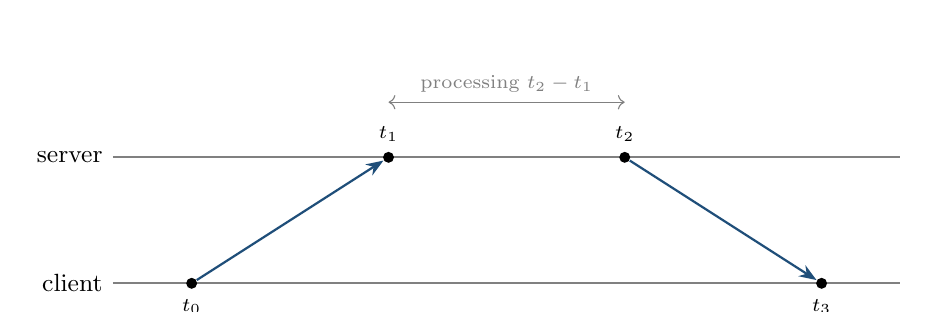
\begin{tikzpicture}[x=1cm,y=1cm]
  \proc{1.6}{server}{10}
  \proc{0}{client}{10}
  \node[ev,label=below:{\scriptsize $t_0$}] (a) at (1,0) {};
  \node[ev,label=above:{\scriptsize $t_1$}] (b) at (3.5,1.6) {};
  \node[ev,label=above:{\scriptsize $t_2$}] (c) at (6.5,1.6) {};
  \node[ev,label=below:{\scriptsize $t_3$}] (d) at (9,0) {};
  \draw[msg] (a) -- (b);
  \draw[msg] (c) -- (d);
  \draw[<->,gray] (3.5,2.3) -- node[above,lbl]{processing $t_2-t_1$} (6.5,2.3);
\end{tikzpicture}
\caption{One NTP exchange. The processing interval is removed from \emph{delay}.}
\end{figure}

\TODO{2--4 sentences in your own words: how the four timestamps improve on Cristian
(Section~\ref{sec:cr-queue}) and what they still cannot fix (asymmetry).}

% ---------------------------------------------------------------------
\subsection{Implementation}
\begin{itemize}[itemsep=2pt]
  \item Offset/delay formulas: \TODO{function} in \src{protocols/ntp/protocol.go}
  \item Minimum-delay filter: \TODO{function}
  \item Stratum / upstream selection: \TODO{function}
  \item RPC wiring: \src{protocols/ntp/rpc.go}; clock model: \src{protocols/ntp/clock.go}
  \item Tests: \src{protocols/ntp/protocol_test.go}
\end{itemize}

\phead{State fields reported}
\begin{table}[H]\centering\small
\begin{tabularx}{\linewidth}{@{}lX@{}}
\toprule
Field & Meaning \\ \midrule
\fld{stratum} / \fld{upstream} & \TODO{} \\
\fld{last.samples}             & \TODO{(per sample: $t_0..t_3$, delay, offset, error)} \\
\fld{last.selected}            & \TODO{(zero-based index; $-1$ = no valid sample)} \\
\fld{lastError}                & \TODO{} \\
\TODO{more}                    & \\
\bottomrule
\end{tabularx}
\end{table}

\phead{Application inputs}
\begin{table}[H]\centering\small
\begin{tabularx}{\linewidth}{@{}llX@{}}
\toprule
Input & Fields & Effect \\ \midrule
\fld{Application.Sync}           & \fld{servers}, \fld{samples}, \fld{processingMS} & \TODO{} \\
\fld{Application.ConfigureClock} & \fld{offsetMS}, \fld{driftPPM} & \TODO{} \\
\fld{Application.Read}           & --- & \TODO{} \\
\bottomrule
\end{tabularx}
\end{table}

% ---------------------------------------------------------------------
\subsection{Scenario coverage}
\begin{table}[H]\centering\small
\begin{tabularx}{\linewidth}{@{}llXl@{}}
\toprule
Report section & Handout & What it shows & Export \\ \midrule
\ref{sec:ntp-normal}  & A         & processing time $t_2-t_1$ is subtracted & \TODO{file} \\
\ref{sec:ntp-filter}  & B         & minimum-delay filtering (8 samples, jitter) & \TODO{file} \\
\ref{sec:ntp-stratum} & C         & error accumulates with stratum & \TODO{file} \\
\ref{sec:ntp-crash}   & (fault A) & upstream crashes & \TODO{file} \\
\ref{sec:ntp-part}    & (fault B) & partition / asymmetric link & \TODO{file} \\
\ref{sec:ntp-variant} & variant   & \TODO{your choice} & \TODO{file} \\
\bottomrule
\end{tabularx}
\end{table}

% ---------------------------------------------------------------------
\scenario{Normal (handout A): server processing time is subtracted}{ntp-normal}
\phead{Setup}
\begin{setuptable}
Nodes / latency & 3 nodes, \TODO{80}\,ms, Docker \\
Input           & node-2: \fld{Sync} \fld{servers=["node-1"]}, \fld{samples=}\fillin, \fld{processingMS=200} \\
Export          & \TODO{} \\
\end{setuptable}
\phead{Steps}
\begin{steps}
  \item \TODO{}
\end{steps}
\phead{Result (one sample)}
\begin{table}[H]\centering\small
\begin{tabular}{@{}rrrrrrr@{}}
\toprule
$t_0$ & $t_1$ & $t_2$ & $t_3$ & $t_2-t_1$ & delay & offset \\ \midrule
\fillin & \fillin & \fillin & \fillin & \fillin & \fillin & \fillin \\
\bottomrule
\end{tabular}
\end{table}
\screenshot{ntp-normal.png}{NTP exchange; the gap on node-1 between receive and reply is the processing time.}
\phead{Explanation}
\TODO{3--5 sentences. Compare the measured send/receive times in the diagram with
$t_0..t_3$; show $t_2-t_1 \approx$ processingMS and that \emph{delay} excludes it.}

% ---------------------------------------------------------------------
\scenario{Handout B: minimum-delay filtering}{ntp-filter}
\phead{Setup}
\begin{setuptable}
Nodes / latency & 3 nodes, \TODO{}\,ms with jitter \TODO{distribution / amount} \\
Input           & \fld{Sync} with \fld{samples=8} \\
Export          & \TODO{} \\
\end{setuptable}
\phead{Result}
\begin{table}[H]\centering\small
\begin{tabular}{@{}rrrl@{}}
\toprule
\# & delay (ms) & offset (ms) & selected? \\ \midrule
0 & \fillin & \fillin & \\
1 & \fillin & \fillin & \\
\multicolumn{4}{c}{\TODO{\dots up to 7}} \\
\bottomrule
\end{tabular}
\end{table}
\screenshot{ntp-filter.png}{Eight samples under jitter.}
\phead{Explanation}
\TODO{3--5 sentences. Why pick the smallest delay and not the smallest offset?}

% ---------------------------------------------------------------------
\scenario{Handout C: error accumulates with stratum}{ntp-stratum}
\phead{Setup}
\begin{setuptable}
Nodes / latency & 3 nodes, \TODO{}\,ms \\
Chain           & node-1 (stratum 1) $\to$ node-2 $\to$ node-3 \\
Export          & \TODO{} \\
\end{setuptable}
\phead{Steps}
\begin{steps}
  \item On node-3, try \fld{Sync} from node-2 \emph{before} node-2 is synchronised (expect failure).
  \item Sync node-2 from node-1, then node-3 from node-2.
  \item \TODO{}
\end{steps}
\phead{Result}
\begin{table}[H]\centering\small
\begin{tabular}{@{}lrlr@{}}
\toprule
Node & stratum & upstream & final \fld{errorMs} \\ \midrule
node-1 & 1 & ---    & \fillin \\
node-2 & \fillin & node-1 & \fillin \\
node-3 & \fillin & node-2 & \fillin \\
\bottomrule
\end{tabular}
\end{table}
\phead{Explanation}
\TODO{3--5 sentences.}

% ---------------------------------------------------------------------
\scenario{Fault A: an upstream server crashes}{ntp-crash}
\phead{Setup and steps}
\begin{steps}
  \item \TODO{e.g.\ crash node-1 and sync node-2 from node-1 (it fails). Then sync
        node-3 from both node-1 and node-2 and show that node-2 still supplies a sample.}
\end{steps}
\screenshot{ntp-crash.png}{\TODO{caption}}
\phead{Explanation}
\TODO{3--5 sentences. Is the clock left unchanged on failure? What does
\fld{selected} show?}

% ---------------------------------------------------------------------
\scenario{Fault B: partition or asymmetric link}{ntp-part}
\phead{Setup and steps}
\begin{steps}
  \item \TODO{e.g.\ set node-2$\to$node-1 = 2000\,ms, node-1$\to$node-2 = 200\,ms and sync;
        compare with Cristian's error in Section~\ref{sec:cr-asym}.}
\end{steps}
\phead{Result}
\TODO{table: predicted bias $(d_\text{fwd} - d_\text{rev})/2$ vs.\ measured}
\phead{Explanation}
\TODO{3--5 sentences. Four timestamps remove server work, but not asymmetric network delay.}

% ---------------------------------------------------------------------
\scenario{Design variant: \TODO{name}}{ntp-variant}
\hint{The handout gives no fixed NTP variant. Ideas: (1) choose the sample with the
smallest |offset| instead of the smallest delay; (2) do not subtract $t_2-t_1$
(i.e.\ fall back to Cristian); (3) average all offsets. Pick one, describe the code
change, and show the error it causes.}
\phead{Code change}
\TODO{what you changed, with a link to the line}
\phead{Result}
\TODO{baseline vs.\ variant, same scenario}
\phead{Explanation}
\TODO{3--5 sentences: why the original design is needed.}

% ---------------------------------------------------------------------
\subsection{Discussion questions}
\begin{qa}{Why pick the smallest delay rather than the smallest offset?}
\TODO{2--4 sentences.}
\end{qa}
\begin{qa}{Why does error accumulate with stratum?}
\TODO{2--4 sentences.}
\end{qa}
\begin{qa}{\TODO{other question}}
\TODO{2--4 sentences.}
\end{qa}

\subsection{Boundaries (what is not implemented)}
\begin{itemize}[itemsep=1pt]
  \item \TODO{e.g.\ no NTP packet format/UDP, no periodic polling, no falseticker
        rejection, steps instead of slewing, no external UTC.}
\end{itemize}

\clearpage
\section{Lamport clocks and vector clocks}\label{sec:lc}
Handout: LAB1 §3.4 \\
Code: \TODO{\src{protocols/logical-clocks} or \src{protocols/lamport}}

% ---------------------------------------------------------------------
\subsection{Algorithm}
Every node $i$ keeps a scalar $L$ and a vector $V$ of length $n$.
\begin{center}\small
\begin{tabular}{@{}lll@{}}
\toprule
Event at node $i$ & Lamport & Vector \\ \midrule
local or send & $L \leftarrow L+1$ & $V[i] \leftarrow V[i]+1$ \\
receive $(L_m, V_m)$ & $L \leftarrow \max(L, L_m)+1$ &
  $V[k] \leftarrow \max(V[k], V_m[k])\ \forall k$, then $V[i] \leftarrow V[i]+1$ \\
\bottomrule
\end{tabular}
\end{center}
Total-order timestamp: \TODO{$L.i$, or $n\cdot L + i$ -- write the one your code uses}.

Properties to verify:
\begin{itemize}[itemsep=1pt]
  \item $e \to e' \Rightarrow L(e) < L(e')$, but not the converse.
  \item $V(e) < V(e') \iff e \to e'$; otherwise the events are concurrent ($e \parallel e'$).
  \item The total order is arbitrary for concurrent events.
\end{itemize}

% ---------------------------------------------------------------------
\subsection{Implementation}
\begin{itemize}[itemsep=2pt]
  \item Clock update rules: \TODO{function names + links}
  \item Message piggybacking (what is sent with each message): \TODO{}
  \item \fld{Compare}: \TODO{where, and what it returns}
  \item Concurrency: \TODO{which mutex protects the clock; see the variant in
        Section~\ref{sec:lc-variant}}
\end{itemize}

\phead{State fields and inputs}
\begin{table}[H]\centering\small
\begin{tabularx}{\linewidth}{@{}lX@{}}
\toprule
Field / input & Meaning \\ \midrule
\TODO{\fld{lamport}}  & \TODO{} \\
\TODO{\fld{vector}}   & \TODO{} \\
\TODO{\fld{events}}   & \TODO{} \\
\TODO{\fld{Local}}    & \TODO{} \\
\TODO{\fld{Send}}     & \TODO{} \\
\TODO{\fld{Compare}}  & \TODO{} \\
\TODO{\fld{Auto}}     & \TODO{} \\
\bottomrule
\end{tabularx}
\end{table}

% ---------------------------------------------------------------------
\subsection{Scenario coverage}
\begin{table}[H]\centering\small
\begin{tabularx}{\linewidth}{@{}llXl@{}}
\toprule
Report section & Handout & What it shows & Export \\ \midrule
\ref{sec:lc-slide}  & A         & lecture slide 37: $L(b) > L(e)$ but $b \parallel e$ & \TODO{file} \\
\ref{sec:lc-equal}  & B         & three concurrent events with equal $L$ & \TODO{file} \\
\ref{sec:lc-auto}   & C         & invariant over random events (\fld{Auto}) & \TODO{file} \\
\ref{sec:lc-crash}  & (fault A) & node crash and recovery & \TODO{file} \\
\ref{sec:lc-part}   & (fault B) & blocked link: send without receive & \TODO{file} \\
\ref{sec:lc-variant}& variant   & \TODO{} & \TODO{file} \\
\bottomrule
\end{tabularx}
\end{table}

% ---------------------------------------------------------------------
\scenario{Normal (handout A): the example on lecture slide 37}{lc-slide}
\phead{Setup}
\begin{setuptable}
Nodes / latency & 3 nodes, \TODO{}\,ms, Docker \\
Export          & \TODO{} \\
\end{setuptable}
\phead{Steps}
\begin{steps}
  \item \TODO{the exact sequence of Local / Send inputs that reproduces the figure}
\end{steps}

\begin{figure}[H]\centering
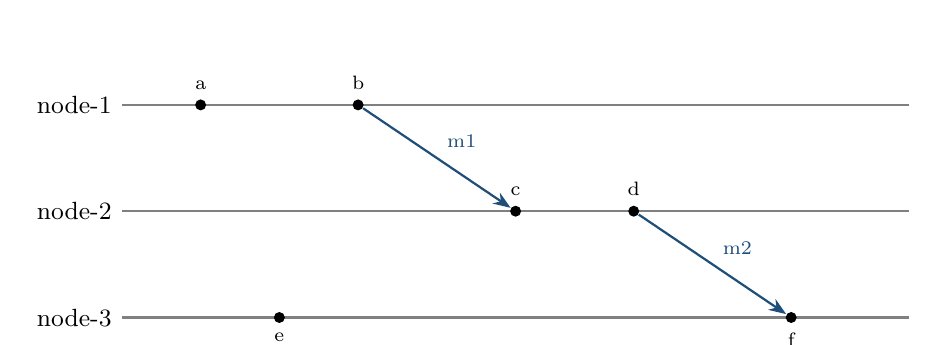
\begin{tikzpicture}[x=1cm,y=0.9cm]
  \proc{3}{node-1}{10}
  \proc{1.5}{node-2}{10}
  \proc{0}{node-3}{10}
  % TODO: adjust positions/labels to match your run
  \node[ev,label=above:{\scriptsize a}] (a) at (1,3) {};
  \node[ev,label=above:{\scriptsize b}] (b) at (3,3) {};
  \node[ev,label=above:{\scriptsize c}] (c) at (5,1.5) {};
  \node[ev,label=above:{\scriptsize d}] (d) at (6.5,1.5) {};
  \node[ev,label=below:{\scriptsize e}] (e) at (2,0) {};
  \node[ev,label=below:{\scriptsize f}] (f) at (8.5,0) {};
  \draw[msg] (b) -- node[lbl,above right]{m1} (c);
  \draw[msg] (d) -- node[lbl,above right]{m2} (f);
\end{tikzpicture}
\caption{Expected event structure (\TODO{check against slide 37}).}
\end{figure}

\phead{Result}
\begin{table}[H]\centering\small
\begin{tabular}{@{}llllrl@{}}
\toprule
Event & Node & Kind & $L$ & $V$ & total order \\ \midrule
a & node-1 & local   & \fillin & \fillin & \fillin \\
b & node-1 & send    & \fillin & \fillin & \fillin \\
c & node-2 & receive & \fillin & \fillin & \fillin \\
d & node-2 & send    & \fillin & \fillin & \fillin \\
e & node-3 & local   & \fillin & \fillin & \fillin \\
f & node-3 & receive & \fillin & \fillin & \fillin \\
\bottomrule
\end{tabular}
\end{table}
\phead{\fld{Compare} results}
\begin{table}[H]\centering\small
\begin{tabular}{@{}llll@{}}
\toprule
Pair & Lamport says & Vector says & Agree? \\ \midrule
$(b, e)$ & \fillin & \fillin & \fillin \\
$(b, f)$ & \fillin & \fillin & \fillin \\
\TODO{} & & & \\
\bottomrule
\end{tabular}
\end{table}
\screenshot{lc-slide37.png}{Space-time diagram reproducing slide 37.}
\phead{Explanation}
\TODO{3--5 sentences. Why $L(b) > L(e)$ does not mean $e \to b$.}

% ---------------------------------------------------------------------
\scenario{Handout B: concurrent events with equal Lamport values}{lc-equal}
\phead{Steps}
\begin{steps}
  \item On a fresh run, have node-1, node-2, node-3 each produce one local event (no messages).
  \item \fld{Compare} each pair.
\end{steps}
\phead{Result}
\TODO{table: three events, $L=1$, vectors, total-order numbers, pairwise comparison}
\phead{Explanation}
\TODO{3--5 sentences. Does the order 1.1 $<$ 1.2 $<$ 1.3 have any physical meaning?}

% ---------------------------------------------------------------------
\scenario{Handout C: invariant after random events}{lc-auto}
\phead{Setup}
\begin{setuptable}
Nodes / latency & \TODO{} \\
Auto settings   & \TODO{rate, duration} \\
Export          & \TODO{} \\
\end{setuptable}
\phead{Result}
\begin{table}[H]\centering\small
\begin{tabular}{@{}lllll@{}}
\toprule
Event 1 & Event 2 & Lamport order & Vector relation & \fld{agrees} \\ \midrule
\fillin & \fillin & \fillin & \fillin & \fillin \\
\fillin & \fillin & \fillin & \fillin & \fillin \\
\fillin & \fillin & \fillin & \fillin & \fillin \\
\bottomrule
\end{tabular}
\end{table}
\phead{Explanation}
\TODO{3--5 sentences. Every causal pair agrees; some Lamport-ordered pairs are concurrent.}

% ---------------------------------------------------------------------
\scenario{Fault A: a node crashes and recovers}{lc-crash}
\phead{Steps}
\begin{steps}
  \item \TODO{produce events, crash node-2, send to it, recover, produce more events}
\end{steps}
\phead{Explanation}
\TODO{3--5 sentences. Are the counters restored (\fld{sdk.Save}/\fld{sdk.Load})?
What would go wrong if a recovered node restarted at $L=0$?}

% ---------------------------------------------------------------------
\scenario{Fault B: blocked link or high latency}{lc-part}
\phead{Steps}
\begin{steps}
  \item \TODO{block node-1$\to$node-2, Send, heal, Send again}
\end{steps}
\phead{Explanation}
\TODO{3--5 sentences. A send event exists without a receive event; the vector
clocks still describe causality correctly.}

% ---------------------------------------------------------------------
\scenario{Design variant: \TODO{name}}{lc-variant}
\hint{The handout gives no fixed variant here. Options: (1) on receive, skip the
$\max$ and just increment -- then $e \to e'$ no longer implies $L(e) < L(e')$;
(2) merge vectors without $\max$ (copy the incoming vector) -- causality is lost;
(3) remove the mutex around the clock (your \nolinkurl{protocols/lamport} code has
this experiment commented in) and show the corrupted state under concurrent sends.}
\phead{Code change}
\TODO{}
\phead{Result}
\TODO{baseline vs.\ variant}
\phead{Explanation}
\TODO{3--5 sentences.}

% ---------------------------------------------------------------------
\subsection{Discussion questions}
\begin{qa}{Why does $L(e) < L(e')$ not imply $e \to e'$?}
\TODO{2--4 sentences.}
\end{qa}
\begin{qa}{Does the total order among concurrent events have physical meaning?}
\TODO{2--4 sentences.}
\end{qa}
\begin{qa}{What does a vector clock cost compared with a Lamport clock?}
\TODO{2--4 sentences (message size $O(n)$, fixed membership).}
\end{qa}

\subsection{Boundaries (what is not implemented)}
\begin{itemize}[itemsep=1pt]
  \item \TODO{e.g.\ fixed membership, no causal-delivery buffer, no total-order broadcast.}
\end{itemize}

\clearpage
\section{Ricart--Agrawala mutual exclusion}\label{sec:ra}
Handout: LAB1 §4.4 \\
Code: \src{protocols/randa}

% ---------------------------------------------------------------------
\subsection{Algorithm}
To enter the critical section (CS), node $i$ stamps a request with its Lamport
timestamp $(L, i)$ and sends \texttt{Request} to all $n-1$ other nodes. It enters
when it has received a \texttt{Reply} from all of them. A node receiving a request:
\begin{itemize}[itemsep=1pt]
  \item replies at once if it is neither holding nor wanting the CS, or if it wants
        the CS but the incoming timestamp is smaller (higher priority);
  \item otherwise \emph{defers} the reply until it leaves the CS.
\end{itemize}
There is no \texttt{Release} message: the deferred replies act as the release.
Messages per CS entry: $2(n-1)$ (Lamport mutual exclusion needs $3(n-1)$).

\TODO{2--4 sentences in your own words: why the timestamp total order prevents
deadlock and guarantees mutual exclusion.}

% ---------------------------------------------------------------------
\subsection{Implementation}
\begin{itemize}[itemsep=2pt]
  \item Lock state machine (indifferent / waiting / holding):
        \texttt{ralock} in \src{protocols/randa/locks.go}
  \item Handling an incoming request (the ``defer'' decision): \texttt{ralock.question}
        in \src{protocols/randa/locks.go}
  \item Broadcasting requests and waiting for all replies: \texttt{ralock.lock}
  \item RPC handlers: \src{protocols/randa/application.go};
        Lamport clock: \src{protocols/randa/clock.go}
  \item \TODO{local lock / how concurrent Acquire on the same node is handled}
\end{itemize}

\phead{State fields reported}
\hint{LAB1 §4 asks all mutual-exclusion protocols to report \fld{role},
\fld{entries}, \fld{lastWaitMs}, \fld{messagesSent}. Make sure randa reports these.}
\begin{table}[H]\centering\small
\begin{tabularx}{\linewidth}{@{}lX@{}}
\toprule
Field & Meaning \\ \midrule
\fld{role}         & \TODO{(released / wanted / critical)} \\
\fld{entries}      & \TODO{} \\
\fld{lastWaitMs}   & \TODO{} \\
\fld{messagesSent} & \TODO{} \\
\fld{deferred}     & \TODO{} \\
\fld{clock}        & \TODO{} \\
\bottomrule
\end{tabularx}
\end{table}

\phead{Application inputs}
\begin{table}[H]\centering\small
\begin{tabularx}{\linewidth}{@{}llX@{}}
\toprule
Input & Fields & Effect \\ \midrule
\TODO{\fld{Application.Acquire}} & \fld{holdMs} & \TODO{} \\
\TODO{\fld{Application.Auto}}    & \TODO{}      & \TODO{} \\
\fld{Application.Lock} / \fld{Unlock} & --- & \TODO{} \\
\bottomrule
\end{tabularx}
\end{table}

% ---------------------------------------------------------------------
\subsection{Scenario coverage}
\begin{table}[H]\centering\small
\begin{tabularx}{\linewidth}{@{}llXl@{}}
\toprule
Report section & Handout & What it shows & Export \\ \midrule
\ref{sec:ra-normal}  & A         & two simultaneous requests & \TODO{file} \\
\ref{sec:ra-crash}   & B         & an uninvolved node crashes, everyone blocks & \TODO{file} \\
\ref{sec:ra-jitter}  & C         & random load, exponential jitter, FIFO vs.\ unordered & \TODO{file} \\
\ref{sec:ra-variant} & variant   & \TODO{} & \TODO{file} \\
\bottomrule
\end{tabularx}
\end{table}

% ---------------------------------------------------------------------
\scenario{Normal (handout A): two nodes request at the same time}{ra-normal}
\phead{Setup}
\begin{setuptable}
Nodes / latency & 3 nodes, \TODO{}\,ms, Docker \\
Input           & node-1 and node-3: \fld{Acquire(holdMs=}\fillin\fld{)} concurrently \\
Export          & \TODO{} \\
\end{setuptable}
\phead{Steps}
\begin{steps}
  \item \TODO{}
\end{steps}
\phead{Result}
\begin{table}[H]\centering\small
\begin{tabular}{@{}lrrrr@{}}
\toprule
Node & request timestamp & entered CS at & \fld{lastWaitMs} & \fld{messagesSent} \\ \midrule
node-1 & \fillin & \fillin & \fillin & \fillin \\
node-3 & \fillin & \fillin & \fillin & \fillin \\
\bottomrule
\end{tabular}
\end{table}
\screenshot{ra-normal.png}{Crossing requests; the higher-priority node replies immediately, the other defers.}
\phead{Explanation}
\TODO{3--5 sentences. Point to the deferred reply in the diagram. Count messages:
is it $2(n-1)$ per entry?}

% ---------------------------------------------------------------------
\scenario{Fault A (handout B): an uninvolved node crashes}{ra-crash}
\phead{Steps}
\begin{steps}
  \item Crash node-2 while it is not requesting the CS.
  \item node-1 calls \fld{Acquire}.
  \item \TODO{recover node-2 and show what happens}
\end{steps}
\screenshot{ra-crash.png}{node-1's request to node-2 is dropped; node-1 never enters.}
\phead{Explanation}
\TODO{3--5 sentences. Why does one crash block everyone? Compare with Lamport
mutual exclusion (same weakness).}

% ---------------------------------------------------------------------
\scenario{Fault B (handout C): random load on an exponentially jittered network}{ra-jitter}
\phead{Setup}
\begin{setuptable}
Nodes / latency & 5 nodes, exponential latency, mean \TODO{}\,ms \\
Load            & \fld{Auto} on all nodes, \TODO{rate / duration} \\
Ordering        & run 1: FIFO (default); run 2: \texttt{"ordering": "unordered"} \\
Export          & \TODO{} \\
\end{setuptable}
\phead{Check}
\fld{atMostOne} on \fld{role == critical} over the whole history
(\src{scripts/scenarios.mjs}): \TODO{pass/fail for each run}.
\phead{Result}
\begin{table}[H]\centering\small
\begin{tabular}{@{}lrrrl@{}}
\toprule
Ordering & CS entries & mean wait (ms) & messages / entry & mutual exclusion held? \\ \midrule
FIFO      & \fillin & \fillin & \fillin & \fillin \\
unordered & \fillin & \fillin & \fillin & \fillin \\
\bottomrule
\end{tabular}
\end{table}
\phead{Explanation}
\TODO{3--5 sentences. Does reordering break mutual exclusion? Why / why not for
\emph{this} implementation (note: RPC request and reply are paired).}

% ---------------------------------------------------------------------
\scenario{Design variant: \TODO{name}}{ra-variant}
\hint{Handout §4.3's variant is the message-count comparison: run the same scenario
on Lamport mutual exclusion (\nolinkurl{protocols/lamport_mutex}) and on R--A and
compare \fld{messagesSent} ($3(n-1)$ vs.\ $2(n-1)$). A stronger variant that shows
\emph{why} a rule is needed: (1) do not defer -- reply immediately even while
holding the CS -- and show two nodes in \fld{role=critical}; or (2) break ties by
something other than (timestamp, node id) and show a deadlock.}
\phead{Code change}
\TODO{}
\phead{Result}
\begin{table}[H]\centering\small
\begin{tabular}{@{}lrrl@{}}
\toprule
Version & $n$ & messages / CS entry & mutual exclusion held? \\ \midrule
Ricart--Agrawala (baseline) & \fillin & \fillin & \fillin \\
\TODO{variant or Lamport ME} & \fillin & \fillin & \fillin \\
\bottomrule
\end{tabular}
\end{table}
\phead{Explanation}
\TODO{3--5 sentences.}

% ---------------------------------------------------------------------
\subsection{Discussion questions}
\begin{qa}{Why does Ricart--Agrawala need only $2(n-1)$ messages while Lamport needs $3(n-1)$?}
\TODO{2--4 sentences.}
\end{qa}
\begin{qa}{Why does a crash of an uninvolved node block everyone?}
\TODO{2--4 sentences.}
\end{qa}
\begin{qa}{Does message reordering break mutual exclusion?}
\TODO{2--4 sentences.}
\end{qa}

\subsection{Boundaries (what is not implemented)}
\begin{itemize}[itemsep=1pt]
  \item \TODO{e.g.\ no failure detection, no persistence, fixed membership.}
\end{itemize}

\clearpage
\section{Summary}

\subsection{Comparison of the three physical-clock / logical-clock approaches}
\begin{table}[H]\centering\small
\begin{tabularx}{\linewidth}{@{}lXXX@{}}
\toprule
 & Cristian & NTP & Lamport / vector \\ \midrule
What it gives       & \TODO{} & \TODO{} & \TODO{} \\
Messages per sync   & \TODO{} & \TODO{} & --- \\
Main error source   & \TODO{} & \TODO{} & --- \\
Effect of a crash   & \TODO{} & \TODO{} & \TODO{} \\
\bottomrule
\end{tabularx}
\end{table}

\subsection{What each design variant taught me}
\begin{itemize}[itemsep=2pt]
  \item \textbf{Cristian:} \TODO{one sentence}
  \item \textbf{NTP:} \TODO{one sentence}
  \item \textbf{Lamport / vector:} \TODO{one sentence}
  \item \textbf{Ricart--Agrawala:} \TODO{one sentence}
\end{itemize}

\subsection{Problems I ran into}
\TODO{Bugs you found while implementing (e.g.\ the race without the mutex in the
Lamport code, the channel-swap race noted in \nolinkurl{randa/locks.go}), and how you
fixed them.}

\subsection{Bonus (optional)}
\TODO{Automated scenarios, tests, tooling, or delete this subsection.}


\appendix
\clearpage
\section{Reproduction index}\label{app:repro}
Every scenario in this report, with where its evidence lives.
Automated scenarios run with
\texttt{node scripts/scenarios.mjs run <protocol> <id>}.
Exported runs are in \src{report}; screenshots are in
\nolinkurl{report/stanleyreport/figures/}.

\begin{table}[H]\centering\small
\begin{tabularx}{\linewidth}{@{}lllX@{}}
\toprule
Protocol & Scenario & \nolinkurl{scenarios.json} id & Exported run (\nolinkurl{report/}) \\ \midrule
Cristian & normal          & \texttt{a-normal}       & \nolinkurl{cristian_scenA_normal.json} \\
Cristian & server crash    & \texttt{b-crash}        & \nolinkurl{cristian_scenB_crash.json} \\
Cristian & asymmetric      & \texttt{c-asymmetric}   & \nolinkurl{cristian_scenC_asymmetric.json} \\
Cristian & server delay    & \texttt{d-server-delay} & \nolinkurl{cristian_scenD_serverDelay.json} \\
Cristian & variant         & \texttt{e-variant}      & \nolinkurl{cristian_designVariant.json} \\
\midrule
NTP & processing time & \TODO{} & \TODO{} \\
NTP & filtering       & \TODO{} & \TODO{} \\
NTP & stratum chain   & \TODO{} & \TODO{} \\
NTP & crash           & \TODO{} & \TODO{} \\
NTP & partition       & \TODO{} & \TODO{} \\
NTP & variant         & \TODO{} & \TODO{} \\
\midrule
Lamport/vector & slide 37     & \TODO{} & \TODO{} \\
Lamport/vector & equal $L$    & \TODO{} & \TODO{} \\
Lamport/vector & Auto         & \TODO{} & \TODO{} \\
Lamport/vector & crash        & \TODO{} & \TODO{} \\
Lamport/vector & blocked link & \TODO{} & \TODO{} \\
Lamport/vector & variant      & \TODO{} & \TODO{} \\
\midrule
R--A & two requests  & \TODO{} & \TODO{} \\
R--A & crash         & \TODO{} & \TODO{} \\
R--A & jitter        & \TODO{} & \TODO{} \\
R--A & variant       & \TODO{} & \TODO{} \\
\bottomrule
\end{tabularx}
\end{table}


\end{document}
